\documentclass[12pt]{article}
\usepackage{hyperref}
\usepackage{listings}
\usepackage[margin=1in]{geometry}
\usepackage{enumitem}
\usepackage{multicol}
\usepackage{array}
\usepackage{titlesec}
\usepackage{helvet}
\renewcommand{\familydefault}{\sfdefault}
\usepackage{amsmath}     % For math equations
\usepackage{amssymb}     % For advanced math symbols
\usepackage{amsfonts} % For math fonts
\usepackage{gvv}
\usepackage{esint}
\usepackage[utf8]{inputenc}
\usepackage{graphicx}
\usepackage{pgfplots}
\pgfplotsset{compat=1.18}
\titleformat{\section}{\bfseries\large}{\thesection.}{1em}{}
\setlength{\parindent}{0pt}
\setlength{\parskip}{6pt}
\usepackage{multirow}
\usepackage{float}
\usepackage{caption}




\begin{document}
\begin{center}
    

\textbf{\Large AI25BTECH11034 - SUJAL CHAUHAN } 
\end{center}
\textbf{Problem 1.8.10}  
Find the distance between the points $(0,5)$ and $(-5,0)$ .



\textbf{Solution.}
let us define our points as $\vec{A} $ and $\vec{B}$
\begin{table}[H]
\centering
\begin{tabular}[12pt]{ |c| c|}
    \hline
    \textbf{Input variable} & \textbf{Value}\\ 
    \hline
    $\vec{A}$ & \myvec{0 \\5 } \\
    \hline 
    $\vec{B}$ & \myvec{-5 \\ 0}\\
    \hline
    \end{tabular}
    \caption{
    \label{}
    }
 \end{table}

Represent the points as vectors:

\begin{align}
 \vec{A}= \myvec{0 \\ 5}, \qquad \vec{B} = \myvec{-5 \\ 0 } 
\end{align}
The distance between $\vec{A}$ and $\vec{B}$ is


\begin{align}
d(\vec{A},\vec{B}) = \|\vec{B} - \vec{A}\| 
\end{align}

Subtracting the vectors,

\begin{align}
\vec{B} - \vec{A} = \myvec{0 \\ 5 } - \myvec{-5 \\ 0} = \myvec{5 \\ 5}
\end{align}


Now, compute the Euclidean norm:

\begin{align}
d(\vec{A},\vec{B}) = \sqrt{(\vec{B}-\vec{A})^T(\vec{B}-\vec{A})}
\end{align}



\begin{align}
d(\vec{A},\vec{B}) = \sqrt{\myvec{5 & 5 }\myvec{5\\ 5}} = \sqrt{50}
\end{align}


\begin{align}
 d(\vec{A},\vec{B}) = 5\sqrt{2}
\end{align}



\textbf{Final Answer:}

\begin{align}
 d(\vec{A},\vec{B}) = \|\vec{B} - \vec{A}\| = 5\sqrt{2}
\end{align}

\begin{figure}[H]
    \centering
    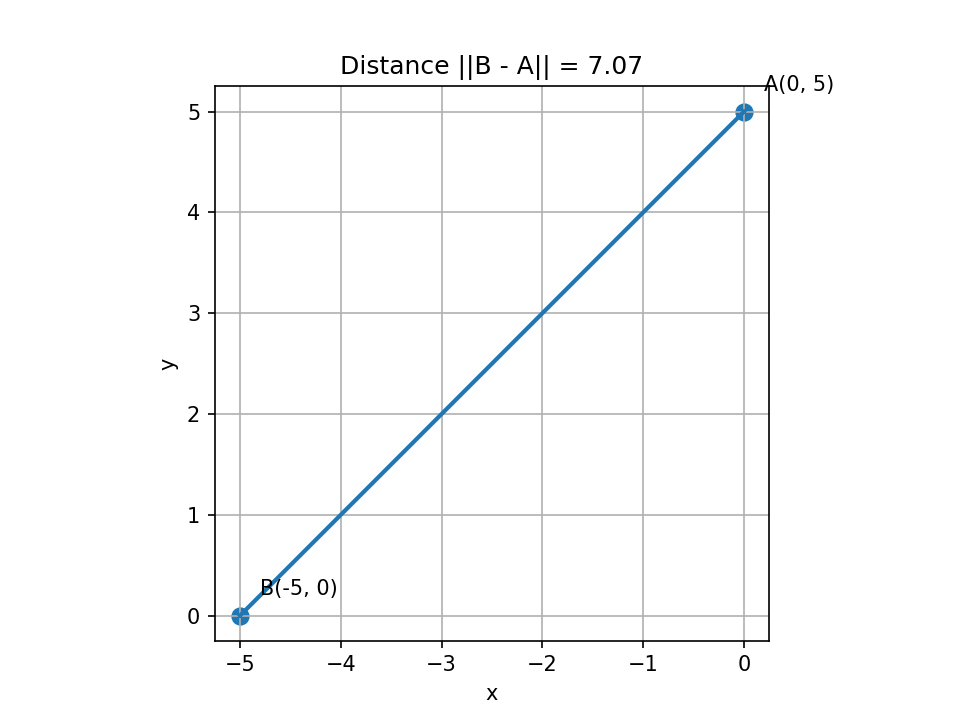
\includegraphics[width=1\columnwidth]{figures/distance.png}
    \caption{}
    \label{fig:placeholder}
\end{figure}


\end{document}